\documentclass[12pt]{article}
%=============
\usepackage{amsmath}
\usepackage{amsfonts}
\usepackage{amssymb}
\usepackage{mathtools}
\usepackage{enumitem}
\usepackage{caption}
\usepackage{xcolor}
%====== commands

\author{Hongli Zhao}
\title{Math 228B: Project 1 Writeup}
\date{\today}
%========= new commands
\newcommand{\intervoo}[2]{(#1, #2)}
\newcommand{\intervcc}[2]{\big[ #1, #2\big]}
\newcommand{\pdx}[1]{\frac{\partial}{\partial {#1}}}
\newcommand{\pddx}[1]{\frac{\partial^2}{\partial {#1}^2}}
\newcommand{\iprod}[1]{\langle {#1}\rangle}
\newcommand{\uno}{\large \textcircled{\small{1}}}
\newcommand{\dos}{\large\textcircled{\small{2}}}
\newcommand{\tres}{\large\textcircled{\small{3}}}
\newcommand{\yonn}{\large\textcircled{\small{4}}} % 4 in Japanese
\newcommand{\cancels}[1]{\underbrace{#1}_\textrm{cancelled}}

%=====begin problem writeup
\begin{document}
\maketitle
\section{2D Poisson problem using 9-point stencil}
\subsection{Defining the transformation to computational domain}

Define the mapping that transforms the original problem defined on $\Omega$, with physical coordinates denoted by $(x,y)$, onto a rectangular domain, $\hat{\Omega}$, with coordinates denoted by $(\xi,\eta)$.

We aim to find a mapping from the computational domain $\intervcc{0}{1}\times \intervcc01$ back to our original domain (the trapezoid). The mapping can be easily inverted, however it is easier to define it from the computational domain first.

We start from the general form for mapping squares to trapezoids:

For the original domain, we have four points:
$$
	P_1 = (0,0)
$$
$$
	P_2 = (\frac12 B, 0)
$$
$$
	P_3 = (A+\frac12 B,H)
$$
$$
	P_4 = (0, H)
$$	

In our computational domain, these points are transformed into:
$$
	\hat{P_1} = (0,0)
$$
$$
	\hat{P_2} = (1,0)
$$
$$
	\hat{P_3} = (1,1)
$$
$$
	\hat{P_4} = (0,1)
$$


To identify the mapping (for both directions), we use a general form:
$$
	\xi(x,y) = a + bx + cy + dxy
$$
$$
	\eta(x,y) = e + fx + gy + hxy
$$ and determine the coefficients $a,b,\cdots,h$. For the inverse direction we can have a similar mapping:
$$
	x(\xi,\eta) = a' + b'\xi + c'\eta + d'\xi\eta
$$
$$
	y(\xi,\eta) = e' + f'\xi + g'\eta + h'\xi\eta
$$

Through plugging in the points $P_i$ and $\hat{P_i}$, we have the mappings to be defined:
$$
	x(\xi,\eta)=\frac{1}{2}B\xi + A\xi\eta
$$
$$
	y(\xi,\eta) = H\eta
$$ which is easily invertible. Giving:
$$
	\xi = \frac{1}{\frac{A}{H}y + \frac{1}{2}B}x = \frac{2Hx}{2Ay+BH}
$$
$$
	\eta = \frac{1}{H}y
$$

\subsection{Second order scheme in computational domain}

In transformed coordinates write down second-order accurate finite difference schemes for the discretization of all the derivative terms in the interior of the domain, as well as for the boundary points. You do not have to derive
special schemes for the corner points: use the left boundary scheme at the corner $P_4$, and $u=0$, at the other three corners.


We can easily express the Laplacian using a chain rule:
$$
	u = u(x,y) = u(x(\xi,\eta),y(\xi,\eta)) = \tilde{u}(\xi,\eta)
$$

Then we can express the second order derivatives in terms of our new coordinates to be solved:

We have:
$$
	\pdx{x} \tilde{u} = \pdx{x} (\tilde{u}_{\xi}\xi_{x} + \tilde{u}_{\eta} \eta_{x})
$$ and:
$$
	\pddx{x} \tilde{u} = \big[\pdx{x} \tilde{u}_{\xi}\big]\cdot \xi_{x} + \tilde{u}_{\xi}\xi_{xx} + \big[\pdx{x} \tilde{u}_{\eta}\big]\eta_{x} + \tilde{u}_{\eta}\eta_{xx}
$$ we can substitute: $\pdx{x} \tilde{u}_{\xi} = \tilde{u}_{\xi\xi}\cdot \pdx{x}\xi, \pdx{x} \tilde{u}_{\eta} = \tilde{u}_{\eta\eta}\cdot \pdx{x}\eta$.


Similarly for the $y$ derivative:
$$
	\pdx{y} \tilde{u} = \pdx{y} (\tilde{u}_{\xi}\xi_{y} + \tilde{u}_{\eta} \eta_{y})
$$ and
$$
	\pddx{y} \tilde{u} = \big[\pdx{y} \tilde{u}_{\xi}\big]\cdot \xi_{y} + \tilde{u}_{\xi}\xi_{yy} + \big[\pdx{y} \tilde{u}_{\eta}\big]\eta_{y} + \tilde{u}_{\eta}\eta_{yy}
$$

we have an explicit formula for the second derivatives:
$$
	{u}_{xx} = \pddx{x} {u} = \tilde{u}_{\xi\xi}\xi_x^2 = \frac{1}{(\frac{A}{H}y + \frac12 B)^2} \tilde{u}_{\xi\xi}
$$
$$
	{u}_{yy} = \pddx{y} {u} = \big[\pdx{y} \tilde{u}_{\xi}\big]\cdot \xi_{y} + \tilde{u}_{\xi}\xi_{yy} + \big[\pdx{y} \tilde{u}_{\eta}\big]\eta_{y} + \tilde{u}_{\eta}\eta_{yy}
$$
$$
	= \big[ \tilde{u}_{\xi\xi}\xi_{y}+\tilde{u}_{\xi\eta} \eta_{y}\big]\eta_{y} + \tilde{u}_{\xi}\xi_{yy}
$$
$$
	= (\eta_{y})^2 \tilde{u}_{\xi\xi} + (\xi_{y}\eta_{y})\tilde{u}_{\xi\eta} + (\xi_{yy})\tilde{u}_{\xi} + \big[ \tilde{u}_{\eta\xi}\xi_{y}+\tilde{u}_{\eta\eta}\eta_{y} \big]\eta_{y}
$$
$$
	= \xi_{y}^2 \tilde{u}_{\xi\xi} + (\eta_{y}^2)\tilde{u}_{\eta\eta} + (2\xi_{y}\eta_{y})\tilde{u}_{\xi\eta} +(\xi_{yy})\tilde{u}_{\xi}
$$

Then the Laplacian is found:
\begin{equation}
	\nabla^2 {u} = {u}_{xx} + {u}_{yy}
	= (\xi_{x}^2 + \xi_{y}^2) \tilde{u}_{\xi\xi} + (\eta_{y}^2)\tilde{u}_{\eta\eta} + (2\xi_{y}\eta_{y})\tilde{u}_{\xi\eta} +(\xi_{yy})\tilde{u}_{\xi}
\end{equation}



From the transformations above in part 1, we can find the derivatives:
$$
	\eta_{x} = \eta_{xx} = 0
$$
$$
	\xi_{x} = \frac{1}{\frac{A}{H}y + \frac{1}{2}B}
$$
$$
	\xi_{xx} = 0
$$
 
$$
	\eta_{y} = \frac1H
$$
$$
	\eta_{yy} = 0
$$
$$
	\xi_{y} = -\frac{4AH}{(2Ay+BH)^2}x
$$
$$
	\xi_{yy} = \frac{16A^2H}{(2Ay+BH)^3}x
$$

Then we need to plug in expressions for $x,y$ in terms of $\xi,\eta$. We have that:
$$
	\xi_{x} = \frac{1}{A\eta+\frac{1}{2}B}
$$
$$
	\xi_{y} = -\frac{4AH(A\eta+\frac{1}{2}B)\xi}{(2AH\eta+BH)^2} = -\frac{4AH(A\eta+\frac{1}{2}B)\xi}{4H^2(AH\eta+\frac12 BH)^2}
$$
$$
	= -\frac{A\xi}{H(A\eta+\frac12 B)}
$$
$$
	\xi_{yy} = \frac{16A^2 H(A\eta+\frac{1}{2}B)\xi}{(2AH\eta+BH)^3} = \frac{16A^2 H(A\eta+\frac{1}{2}B)\xi}{8H^3(A\eta+\frac12 B)^3}
$$
$$
	= \frac{2A^2\xi}{H^2(A\eta+\frac{1}{2}B)^2}
$$


We have transformed our Poisson equation to:
$$
	D_1(\xi,\eta)\tilde{u}_{\xi\xi} + D_2(\xi,\eta)\tilde{u}_{\eta\eta} + D_3(\xi,\eta)\tilde{u}_{\xi\eta}+D_4(\xi,\eta)\tilde{u}_{\xi} = -1
$$ on the computational domain.

We have:
$$
	D_1 = \xi_{x}^2 + \xi_{y}^2 = \frac{H^2+A^2\xi^2}{H^2(A\eta + \frac12 B)^2}
$$
$$
	D_2 \equiv \frac{1}{H^2}, D_3 = -\frac{2A\xi}{H^2(A\eta + \frac12 B)}
$$ and
$$
	D_4 = \eta_{yy} = \frac{2A^2\xi}{H^2(A\eta+\frac{1}{2}B)^2}
$$


\subsubsection{transforming the boundary conditions}
For the Dirichlet boundary conditions, we can directly transform:
$$
	\tilde{u} = 0
$$ for $P_1P_2, P_2P_3$,

For the Neumann boundary condition on $P_1P_4$:
$$
	\pdx{n}u = \iprod{u_x,u_y} \cdot \iprod{-1,0} = -u_x = 0
$$ namely:
$$
	u_x = \tilde{u}_{\xi} \cdot \xi_{x} + \tilde{u}_{\eta} \cdot \eta_{x} = \tilde{u}_{\xi}\cdot \xi_{x} = 0
$$

Giving us:
$$
	\tilde{u}_{\xi} = 0
$$ on $P_1P_4$.


And also on boundary $P_3P_4$, we have:
$$
	\pdx{n}u = \iprod{u_x,u_y} \cdot \iprod{0,1} = u_y = 0
$$ namely:
$$
	u_y = \tilde{u}_{\xi}\cdot \xi_{y} + \tilde{u}_{\eta}\cdot \eta_{y} = 0
$$

Giving us another condition:
$$
	\tilde{u}_{\eta} = \frac{A\eta}{A\eta+\frac{1}{2}B}\tilde{u}_{\xi}
$$
\subsubsection{deriving the scheme}
We divide the scheme into parts (for each boundary and then for the general points in the middle. After space discretization in both $\xi,\eta$ directions, let $U_{i,j}$ denote the computed solution on mesh grid $(i,j) \in \{ 1,2,\cdots,n+1\} \times \{ 1,2,\cdots,n+1\}$, corresponding to $\xi_i, \eta_j$. 
\subsubsection{scheme on $P_1P_2$ and $P_2P_3$}

Due to the Dirichlet boundary condition, we have:
$$
	U_{ij} = 0
$$ for all $j=1, i=1:n+1$. and for $i = n+1, j=2:n+1$.

\subsubsection{scheme on $P_1P_4$}\label{section:3pntstencil}
On $P_1P_4$, we are subject to the Neumann condition:
$$
	\tilde{u}_{\xi} = 0
$$ for $i = 1, j=2:n+1$ on the left boundary.
To calculate the unknown data at $U_{ij}$ we use the data at $U_{(i+1)j}, U_{(i+2)j}$ to be second order accurate.

The derivation uses method of undetermined coefficients. We would like to find an approximation for $\tilde{u}_{\xi}$ by using data points $U_{ij},U_{(i+1)j},U_{(i+2)j}$. We can set up the equations as:
$$
	D_2u({\xi}) = a U(\xi_i, \eta_j) + bU(\xi_i+\Delta \xi,\eta_{j})+ cU(\xi_i+2\Delta\xi,\eta_{j})
$$ by means of Taylor expansion we can derive the appropriate coefficients for a second order approximation to $\tilde{u}_{\xi}$:
$$
	= aU + b(U + h U' + \frac12 h^2 U'' + O(h^3)) + c(U + 2hU' + \frac{(2h)^2}{2}U'' + O(h^3))
$$ 
$$
	= (a+b+c)U + h(b+2c)U' + h^2(\frac{b}{2}+2c)U'' + O(h^3)
$$ where $U = U(\xi_{i},\eta_{j})$, $h = \Delta\xi$, using a shorthand notation.

Let:
$$
	a+b+c = 0
$$
$$
	h(b+2c) = 1
$$
$$
	h^2(\frac{b}{2}+2c) = 0
$$ we can arrive at a second order in $\Delta \xi$ approximation.

Giving us a 3-point stencil:
$$
	D_2u_{\xi} = -\frac{1}{h}(\frac32 U_{ij} - 2U_{(i+1)j} + \frac12 U_{(i+2)j}) = 0
$$ by the Neumann condition. On the computational domain, for $j = 2:n+1$.
\subsubsection{scheme on $P_3P_4$}

On the top of our computational domain, we are subject to the Neumann condition:
$$
	\tilde{u}_{\eta} = \frac{A\eta}{A\eta+\frac{1}{2}B}\tilde{u}	_{\xi}
$$ we can use a similar approach to derive a 5-point stencil for approximating this relation.
$$
	(A\eta+\frac12 B)\tilde{u}_{\eta} = A\eta \tilde{u}_{\xi}
$$

For approximation of $\tilde{u}_{\eta}$ at point $(\xi_{i}, \eta_{j})$, the accessible data points are $U_{(i+1)j},U_{(i-1)j}$, then let:
$$
	\tilde{u}_{\eta} = aU_{(i+1)j} + bU_{(i-1)j}
$$ by Taylor expansion:
$$
	= a(U+hU'+\frac{h^2}{2}U''+O(h^3)) + b(U-hU'+\frac{h^2}{2}U''+O(h^3))
$$
$$
	= (a+b)U + h(a-b)U' + \frac{1}{2}h^2 (a+b) U'' + O(h^3)
$$

Letting:
$$
	a + b = 0
$$
$$
	a - b = 1
$$ we will have a second order scheme for approximating $\tilde{u}_{\eta}$ with $a=-b=\frac12$.

For the other derivative we let:
$$
	\tilde{u}_{\xi} = aU_{ij} + bU_{i(j-1)} + cU_{i(j-2)}
$$ we have the vertical points $U_{i(j+1)}, U_{ij}, U_{i(j-1)}$ as our data for the approximation, and since this is a 3-point stencil, we expect that it is symmetric to Section~\ref{section:3pntstencil} which gives the approximation:
$$
	\tilde{u}_{\xi} = \frac{3}{2}U_{ij} - 2U_{i(j-1)} + \frac12 U_{i(j-2)}
$$

Putting the approximations together, we have a 5-point stencil for this Neumann condition:
$$
	\frac{A\xi_{i}}{2}\big[ U_{(i+1)j} - U_{(i-1)j}\big] - (A\eta_{j}+\frac{B}{2})\big[ \frac32 U_{ij} - 2 U_{i(j-1)} + \frac12 U_{i(j-2)}\big] = 0
$$ which is spatially dependent on $\xi_{i},\eta_{j}$, for $j=n+1,i=2:n$.


\subsubsection{general scheme on the grid}
Now that we have schemes defined on the boundaries, we can now approach the scheme for a general point $(\xi,\eta)$ on the computational domain, which uses a 9-point stencil.

Recall the general formula for the Laplacian on a general point $(\xi,\eta)$:
$$
	D_1(\xi,\eta)\tilde{u}_{\xi\xi} + D_2(\xi,\eta)\tilde{u}_{\eta\eta} + D_3(\xi,\eta)\tilde{u}_{\xi\eta}+D_4(\xi,\eta)\tilde{u}_{\xi} = -1
$$ with spatially dependent coefficients $D_1,D_3,D_4$. Now we need to derive schemes to compute $\tilde{u}_{\xi\xi}, \tilde{u}_{\eta\eta}, \tilde{u}_{\xi\eta}, \tilde{u}_{\xi}$.

For the second derivatives, we use central differencing to achieve second order accuracy; and for the mixed derivative, we can use a 4-point stencil. The schemes are:
$$
	\tilde{u}_{\xi\xi} = \frac{1}{\Delta\xi^2}\big[U_{(i+1)j} - 2U_{ij} + U_{(i-1)j}\big]
$$ similarly:
$$
	\tilde{u}_{\eta\eta} = \frac{1}{\Delta\eta^2}\big[U_{i(j+1)} - 2U_{ij} + U_{i(j-1)}\big]
$$

For the mixed derivative:
$$
	\tilde{u}_{\xi\eta} = \frac{1}{4\Delta\xi\Delta\eta} 
	\big[
		U_{(i+1)(j+1)} - U_{(i+1)(j-1)} - U_{(i-1)(j+1)} + U_{(i-1)(j-1)}
	\big]
$$

Lastly we have:
$$
	\tilde{u}_{\xi} = \frac{1}{2\Delta\xi}(U_{(i+1)j} - U_{(i-1)j})
$$

	Combining the terms, we have a 9-point stencil for a general point on the computational grid.
$$
	\frac{D_1(\xi,\eta)}{\Delta\xi^2}\big[U_{(i+1)j} - 2U_{ij} + U_{(i-1)j}\big] + 
	\frac{D_2(\xi,\eta)}{\Delta\eta^2}\big[U_{i(j+1)} - 2U_{ij} + U_{i(j-1)}\big] 
$$
$$
+ 
	\frac{D_3(\xi,\eta)}{4\Delta\xi\Delta\eta} 
	\big[
		U_{(i+1)(j+1)} - U_{(i+1)(j-1)} - U_{(i-1)(j+1)} + U_{(i-1)(j-1)}
	\big] 
$$
$$
	+ 
	\frac{D_4(\xi,\eta)}{2\Delta\xi}(U_{(i+1)j} - U_{(i-1)j})
	= -1
$$


\subsection{Evaluating the Numerical Integral on the Computational Domain}

For second order accuracy, we use trapezoidal numerical integration. The integral over our computational domain is formulated as follows via the change of variable.

By a change of variable from $(x,y)$ for the integral to be evaluated on the computational domain.
$$
	\int_{\phi(x,y)}u(x,y)dxdy = \int_{\hat{\phi}(\xi,\eta)} u(\xi,\eta) \det{(D\hat{\phi})}(\xi,\eta)d\xi d\eta = \hat{Q}
$$ where $\phi(x,y),\hat{\phi}(\xi,\eta)$ represent the physical and the computational domain.

We have by inverting the mapping:
$$
	\begin{cases}
		x = (A\eta + \frac{B}{2})\xi \\
		y = H\eta
	\end{cases}
$$

Then the Jacobian for our change of variable is:
$$
	\mathcal{J} =
	\begin{pmatrix}
		x_{\xi} = A\eta + \frac{B}{2} & x_{\eta} = A\xi \\
		y_{\xi} = 0 & y_{\eta} = H
	\end{pmatrix}
$$ then we have $\det{(\mathcal{J})} = H\big[ A\eta + \frac{B}{2}\big]$

Finally we can evaluate:
$$
	\hat{Q} = \int_{\bar{B}} H\big[ A\eta + \frac{B}{2} u(\xi,\eta) d\xi d\eta \big]
$$ for $\bar{B}$ our computational domain.
\subsection{Numerical solution contour and 3D plots}
After computing the numerical solution to the PDE, we generate contour plots in both 2D and 3D, and both physical and computational domain (figure 1):
\begin{figure}[h]
	\centering
	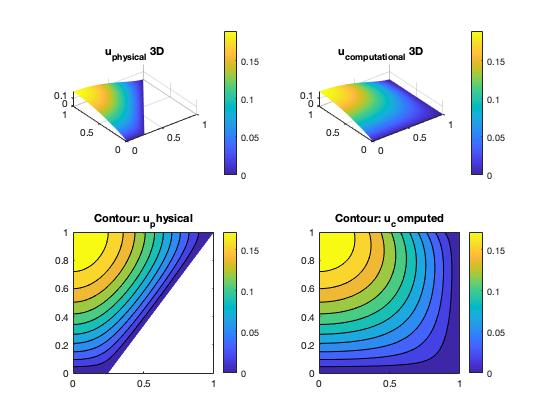
\includegraphics[width=1\linewidth]{./solution_2d_3d.jpg}
	\caption{numerical solution contour plots}
\end{figure}

\subsection{Error plotting}
We plot the errors from both evaluating the solution and evaluation the integral $Q$ and verify that they are indeed second order accurate by a log-log plot. For numerical integration, we use trapezoidal rule (figure 2).
\begin{figure}[h]
	\centering
	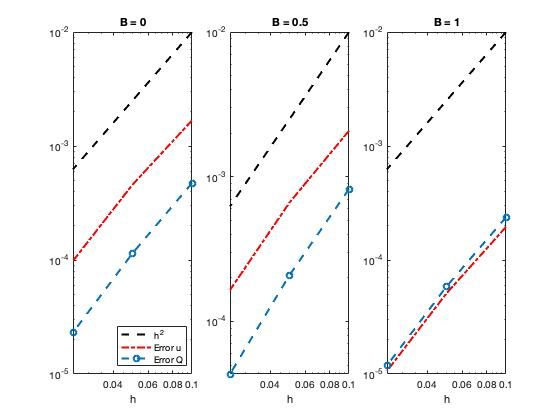
\includegraphics[width=1\linewidth]{./errors.jpg}
	\caption{log-log errors, labelled}
\end{figure}




\section{Local Truncation Error Analysis for $\theta$-stepping}
We derive the local truncation error by applying the scheme on our exact solution $u(x,t)$. Let also $k = \Delta t$, $h = \Delta x$. For simplicity call $c = \gamma$.
\newcommand{\bk}{\kappa}
Then we have:
$$
	u(x,t+k) = u(x,t)+...
$$
$$
\frac{k}{2h^2}\bk
\big[
		u(x-h,t)-2u(x,t)+u(x+h,t) +
	u(x-h,t+k)-2u(x,t+k)+u(x+h,t+k)
	\big]
$$
$$
	-
	kc \big[
		(1-\theta)u(x,t)+\theta u(x,t+k)
	\big]
$$

By rearranging,
$$
	\underbrace{\frac{u(x,t+k) - u(x,t)}{k}}_\textrm{\uno} =
$$
$$
	\frac{1}{2h^2}\bk
\big[
		\underbrace{u(x-h,t)-2u(x,t)+u(x+h,t)}_\textrm{\dos} 
$$
$$
	+
	\underbrace{u(x-h,t+k)-2u(x,t+k)+u(x+h,t+k)}_\textrm{\tres}
	\big]
$$
$$
	-
	c \big[
		\underbrace{(1-\theta)u(x,t)+\theta u(x,t+k)}_\textrm{\yonn}
	\big]
$$ for simplicity, we label these expressions.

Then we have local truncation error defined as:
$$
	\tau(x,t)=\tau
	= \uno - \frac{1}{2h^2}\bk (\dos + \tres) + c\yonn
$$

We begin our Taylor expansion, divided into sections, and revisit $\tau$ when we are done. For simplicity for notations, we let $u(x,t)$ be denoted by $u$, and $u_x$ denotes partial derivative.
\subsection{expansion: \uno}
\uno
$$
	= \frac{1}{k}(u+ku_t+\frac12 k^2u_{tt}+O(k^3)-u)
	= \frac{1}{k}(ku_t+\frac12 k^2u_{tt}+O(k^3))
$$
$$
	= u_t + \frac12 ku_{tt} + O(k^2)
$$
\subsection{expansion: \dos}
\dos
$$
	= \cancels{u - hu_x} + \frac12 h^2u_{xx} \cancels{- \frac16 h^3 u_{xxx}} + O(h^4) \cancels{- 2u + u + hu_x} 
$$
$$
	+ \frac12 h^2 u_{xx} + \cancels{\frac16 h^3 u_{xxx}} + O(h^4)
$$
$$
	= h^2u_{xx}+O(h^4)
$$

\subsection{expansion: \tres}
\tres
$$
	= h^2u_{xx}(x,t+k) + O(h^4), \text{ ( expansion in space should follow that of \dos )}
$$
$$
	= h^2(u_{xx} + ku_{xxt} + O(k^2)) + O(h^4)
$$
$$
	= h^2u_{xx} + h^2ku_{xxt} + O(h^2k^2 + h^4)
$$
\subsubsection{combine \dos and \tres}
\dos $+$\tres
$$
	= 2h^2u_{xx} + h^2ku_{txx} + O(h^2k^2 + h^4)
$$

\subsection{expansion: \yonn}
\yonn
$$
	= u - \theta u + \theta(u + ku_t + O(k^2))
	= u \cancels{- \theta u + \theta u} + \theta ku_t + O(k^2)
$$
$$
	= u + k\theta u_t + O(k^2)
$$

\subsection{collect \uno,\dos,\tres,\yonn}
We revisit our $\tau$:
$$
	\tau = u_t + \frac12 ku_{tt} + O(k^2) - \frac{1}{2h^2} \bk \big[ 2h^2 + h^2ku_{txx} + O(h^2k^2+h^4)\big]
$$
$$
	+ c\big[u+k\theta u_t + O(k^2) \big]
$$
$$
	= u_t + \frac12 ku_{tt} - \frac{1}{2h^2}\bk \big[ 2h^2u_{xx} + h^2ku_{txx} + O(h^2k^2+h^4)\big] + cu + \theta k (cu_t) + O(k^2)
$$
$$
	= u_t + \big[ \frac{1}{2}u_{tt} \big] - \big[ \bk u_{xx} \big] - k\big[ \frac12 \bk u_{txx} \big] + cu + k\big[ \theta cu_t \big] + O(h^2+k^2)
$$

We use the PDE identities:
$$
	\begin{cases}
		\bk u_{xx} = u_t + cu \\
		\bk u_{txx} = u_{tt} + cu_t
	\end{cases}
$$ substituting in:
$$
	\tau =
	\cancels{u_t + k \big[ \frac12 u_{tt} \big] - u_t - cu - k\big[ \frac12 (u_{tt} + cu_t) \big] + cu} + k\big[ \theta cu_t \big] + O(h^2 + k^2)
$$
$$
	= - k \big[ \frac12 cu_t \big] + k \big[ \theta cu_t \big] + O(h^2 + k^2)
$$

Then it is easy to see that:
$$
	\tau = 
	\begin{cases}
		O(h^2 + k^2), \text{ for $\theta = \frac12$} \\
		O(h^2 + k), \text{ for $\theta = 1$} \\
	\end{cases}
$$








%========
\end{document}